\documentclass[a4paper,french,bookmarks]{book}

\usepackage{booktabs}
\usepackage{minitoc}
\usepackage{Structure/4PE18TEXTB}
\usepackage{pdfpages}

\newboxans
\renewcommand{\questionsdecours}{\section*{\centering\EBGaramond\Large Questions~ de~ cours}}
\renewcommand{\thechapter}{\Roman{chapter}}
\renewcommand{\thesubsection}{Exercice \arabic{subsection}}
\setcounter{secnumdepth}{5}
\setcounter{tocdepth}{0}
\mtcsettitle{minitoc}{}
%\renewcommand{\thesection}{\hspace{-11pt}}
%\renewcommand{\thesubsection}{}

\newcommand{\chaptertoc}[0]{
    \setcounter{minitocdepth}{4}
    \begin{tcolorbox}[
        enhanced,
        frame hidden,
        sharp corners,
        detach title,
        spread outwards     = 5pt,
        halign              = center,
        valign              = center,
        borderline west     = {3pt}{0pt}{main20!50!main2!95!gray!90},
        coltitle            = main20!50!main2!95!gray!90, 
        interior style      = {
            left color      = main1white2!65!gray!11,
            middle color    = main1white2!50!gray!10,
            right color     = main1white2!35!gray!9
        },
        arc                 = 0 cm,
        title               = SOMMAIRE,
        fonttitle           = \bfseries\sffamily,
        overlay             = {
            \node[rotate=90, minimum width=1cm, anchor=south,yshift=-0.8cm] at (frame.west) {\tcbtitle};
        }
    ]
        \begin{minipage}{0.83\linewidth}
            \sffamily
            \minitoc
        \end{minipage}
    \end{tcolorbox}
}

\begin{document}
    
    %==============================
    % METADONNEES
    %==============================
    
    \title{TD de Physique de MPI/MPI* (2022-2023)}
    \author{SIAHAAN--GENSOLLEN Rémy}
    \date{\today}
    \hypersetup{
        pdftitle={TD de Physique de MPI/MPI* (2022-2023)},
        pdfauthor={SIAHAAN--GENSOLLEN Rémy},
        pdflang={fr-FR},
        pdfsubject={MPI/MPI*, TD de Physique},
        pdfkeywords={MPI/MPI*, TD de Physique, 2022-2023}
        pdfstartview=
    }
    
    %==============================
    % MISE EN PAGE
    %==============================
    
    \titleformat{\chapter}[display]{\normalfont\huge\bfseries}{}{0pt}{
        \begin{tcolorbox}[
            enhanced,
            frame hidden,
            sharp corners,
            spread sidewards    = 5pt,
            halign              = center,
            valign              = center,
            interior style      = {color=main10!20},
            arc                 = 0 cm,
            fontupper           = \color{black}\sffamily\bfseries\huge,
            fonttitle           = \normalfont\color{white}\sffamily\small,
            top                 = 1cm, 
            bottom              = 0.7cm,
            title               = Chapitre \thechapter,
            attach boxed title to bottom center = {
                yshift=\tcboxedtitleheight/2,
            },
            boxed title style = {
                frame code={
                \path[left color=main21!95!gray!90,right color=main21!95!gray!90] 
                    ([xshift=-10mm]frame.north west) -- 
                    ([xshift=10mm]frame.north east) -- 
                    ([xshift=10mm]frame.south east) -- 
                    ([xshift=-10mm]frame.south west) -- 
                    cycle;
                },
                interior engine=empty
            }
        ]
            #1
        \end{tcolorbox}%
    }
    \titlespacing*{\chapter}{0pt}{-120pt}{-15pt}
    \titleformat{name=\chapter,numberless}[display]{\normalfont\huge\bfseries}{}{0pt}{
        \begin{tcolorbox}[
            enhanced,
            frame hidden,
            sharp corners,
            spread sidewards    = 5pt,
            halign              = center,
            valign              = center,
            interior style      = {color=main10!20},
            arc                 = 0 cm,
            outer arc           = 0pt,
            leftrule            = 0pt,
            rightrule           = 0pt,
            fontupper           = \color{black}\sffamily\bfseries\huge,
            enlarge left by     = -1in-\hoffset-\oddsidemargin, 
            enlarge right by    = -\paperwidth+1in+\hoffset+\oddsidemargin+\textwidth,
            width               = \paperwidth, 
            left                = 1in+\hoffset+\oddsidemargin, 
            right               = \paperwidth-1in-\hoffset-\oddsidemargin-\textwidth,
            top                 = 1cm, 
            bottom              = 1cm
        ]
            #1
        \end{tcolorbox}%
    }
    \titlespacing*{name=\chapter,numberless}{0pt}{-115pt}{0pt}
    
    %==============================
    % PREMIERE DE COUVERTURE
    %==============================

    %
\includepdf[pages={1},scale=1.15,offset=0mm -18mm]{LDCCover.pdf}
    
    %==============================
    % PAGE VIDE
    %==============================
    
    %\pagestyle{empty}
    
    %==============================
    % PAGE DE COUVERTURE INTERNE
    %==============================
    
    \begin{titlepage}
	    \begin{center}
	        {\scshape SIAHAAN--GENSOLLEN Rémy\par}
	        \vspace{2cm}
	        {\huge\sffamily TD de\par}
	        \vspace{0.5cm}
	        {\Huge\bfseries\sffamily PHYSIQUE\par}
	        \vspace{1cm}
	        {\Large\textit{donné pendant mon année de \textsf{MPI/MPI*} à
	        Janson-de-Sailly}\\[5pt]\texttt{(2022-2023)}\par}
	        \vfill
	        {\large\EBGaramond Dernière compilation le \today\par}
        \end{center}
    \end{titlepage}
    
    %==============================
    % PAGE VIDE
    %==============================
    
    \pagestyle{empty}\text{}\newpage
    
    %==============================
    % STYLE DES EN-TÊTES ET PIEDS DE PAGES
    %==============================
    
    \renewcommand\chaptermark[1]{\markboth{#1}{}}
    
    \fancypagestyle{intro}{
        \fancyhf{}
        \renewcommand{\headrulewidth}{0pt}
        \renewcommand{\footrulewidth}{0pt}\fancyfoot[RO,LE]{\GillSansMTMedium\color{white5}\thepage\;/\;\pageref{LastPage}}
        \fancyhead[LE]{\GillSansMTMedium\color{white5}\bfseries TD DE PHYSIQUE}
        \fancyhead[RE]{\GillSansMTMedium\color{white5}Avant-propos}
        \fancyhead[LO]{\GillSansMTMedium\color{white5}\rightmark}
        \fancyhead[RO]{\GillSansMTMedium\color{white5}\textbf{MPI/MPI*} 2022-2023 \quad Janson-de-Sailly}
    }
    
    \fancypagestyle{toc}{
        \fancyhf{}
        \renewcommand{\headrulewidth}{0pt}
        \renewcommand{\footrulewidth}{0pt}\fancyfoot[RO,LE]{\GillSansMTMedium\color{white5}\thepage\;/\;\pageref{LastPage}}
        \fancyhead[LE]{\GillSansMTMedium\color{white5}\bfseries TD DE PHYSIQUE}
        \fancyhead[RE]{\GillSansMTMedium\color{white5}Table des matières}
        \fancyhead[LO]{\GillSansMTMedium\color{white5}\rightmark}
        \fancyhead[RO]{\GillSansMTMedium\color{white5}\textbf{MPI/MPI*} 2022-2023 \quad Janson-de-Sailly}
    }
    
    \fancypagestyle{plain}{
        \fancyhf{}
        \renewcommand{\headrulewidth}{0pt}
        \renewcommand{\footrulewidth}{0pt}\fancyfoot[RO,LE]{\GillSansMTMedium\color{white5}\thepage\;/\;\pageref{LastPage}}
        \fancyhead[LE]{\GillSansMTMedium\color{white5}\bfseries TD DE PHYSIQUE}
        \fancyhead[RE]{\GillSansMTMedium\color{white5}Chapitre \thechapter : \nouppercase{\leftmark}}
        \fancyhead[LO]{\GillSansMTMedium\color{white5}\nouppercase{\rightmark}}
        \fancyhead[RO]{\GillSansMTMedium\color{white5}\textbf{MPI/MPI*} 2022-2023 \quad Janson-de-Sailly}
    }
    
    %==============================
    % PREFACE 
    %==============================
    
    \chapter*{Avant-propos}
    \thispagestyle{intro}
    \addcontentsline{toc}{chapter}{Avant-propos}
    
    \text{\Large\EBGaramond\itshape À tout lecteur potentiel, quelques mots...}\newline\newline\newline
    
    \begin{center}
        \begin{minipage}{0.85\linewidth}
            \large \qquad Ce livre contient la résolution des exercices de TD donnés pendant les cours de physique de mon année de MPI/MPI*. Il vient en complément du livre de cours associé.\newline\newline\newline\text{}
        \end{minipage}
    \end{center}
    
    \hfill{\large\textsc{Siahaan--Gensollen Rémy}}
    
    \pagestyle{intro}
    
    %==============================
    % TABLE DES MATIERES
    %==============================
    
    \newpage
    \dominitoc\nomtcrule 
    {\sffamily\tableofcontents}\mtcaddchapter\pagestyle{toc}
    
    \cleardoublepage
    
    %==============================
    % COURS
    %==============================
    
    \pagestyle{plain}
    
    \chapter{Quelques notions indispensables}
    
    \subsection{}
    
    Calculer pour un gaz parfait la quantité :
    %
    \[ \dep{\dfrac{\partial V}{\partial T}}_P \dep{\dfrac{\partial T}{\partial P}}_V \dep{\dfrac{\partial P}{\partial V}}_T\]
    
    \noafter
    %
    \boxans{
        L'équation des gaz parfaits donne $PV = nRT$. Pour $n$ donné et puisque $R$ est une constante, on a donc :
        %
        \[ V\p{P, T} = \dfrac{nRT}{P} \qquad T\p{P, V} = \dfrac{PV}{nR} \qquad P\p{V, T} = \dfrac{nRT}{V}\]
        %
        Ainsi on a :
        %
        \[ \dep{\dfrac{\partial V}{\partial T}}_P = \dfrac{nR}{P}\qquad \dep{\dfrac{\partial T}{\partial P}}_V = \dfrac{V}{nR} \qquad \dep{\dfrac{\partial P}{\partial V}}_T = -\dfrac{nRT}{V^2}\]
        %
        On multiplie donc pour obtenir :
    }
    %
    \nobefore\yesafter
    %
    \boxansconc{
        \[ \dep{\dfrac{\partial V}{\partial T}}_P \dep{\dfrac{\partial T}{\partial P}}_V \dep{\dfrac{\partial P}{\partial V}}_T = \dfrac{nR}{P}\dfrac{V}{nR}\p{-\dfrac{nRT}{V^2}} = -\dfrac{nRT}{PV} = -1 \]
    }
    %
    \yesbefore
    
    \subsection{}
    
    La force $\vec{F}$ s'exprime dans le repère $\p{\vec{e_x}, \vec{e_y}, \vec{e_z}}$ de la façon suivante : \quad $\vec{F} = \left(\begin{array}{c}
        x  \\
        z^2 y \\
        y^2 z + C
    \end{array}\right)$.
    %
    \begin{enumerate}
        \item Est-ce une force conservative ?
        
        \noafter
        %
        \boxans{
            Soit $\delta W_{\vec{F}} = \vec{F} \cdot \dif \vec{OM}$. On cherche à savoir s'il existe une fonction $E_\text p$ telle que $\delta W_{\vec{F}} = -\dif E_\text p$.
            
            Posons les composantes $F_x = \vec{F} \cdot \vec{e_x}$, $F_y = \vec{F} \cdot \vec{e_y}$ et $F_z = \vec{F} \cdot \vec{e_z}$. L'énoncé amène :
            %
            \[ F_x\p{x, y, z} = x \qquad F_y\p{x, y, z} = z^2y \qquad F_z\p{x, y, z} = y^2z + C \]
            %
            On a donc $\delta W_{\vec{F}} = F_x\p{x, y, z}\dif x + F_y\p{x, y, z}\dif y + F_z\p{x, y, z}\dif z$.
            
            \begin{enumerate}
                \begin{minipage}{0.48\linewidth}
                    \itt $\dep{\dfrac{\partial F_x}{\partial y}}_{x, z} = 0$
                    
                    \itt $\dep{\dfrac{\partial F_x}{\partial z}}_{x, y} = 0$
                    
                    \itt $\dep{\dfrac{\partial F_y}{\partial z}}_{x, y} = 2yz$
                \end{minipage}
                %
                \hfill
                %
                \begin{minipage}{0.48\linewidth}
                    \itt $\dep{\dfrac{\partial F_y}{\partial x}}_{y, z} = 0$
                    
                    \itt $\dep{\dfrac{\partial F_z}{\partial x}}_{y, z} = 0$
                    
                    \itt $\dep{\dfrac{\partial F_z}{\partial y}}_{x, z} = 2yz$
                \end{minipage}
            \end{enumerate}
            %
            On remarque que $\dep{\dfrac{\partial F_x}{\partial y}}_{x, z} = \dep{\dfrac{\partial F_y}{\partial x}}_{y, z}$, que $\dep{\dfrac{\partial F_x}{\partial z}}_{x, y} = \dep{\dfrac{\partial F_z}{\partial x}}_{y, z}$, et que $\dep{\dfrac{\partial F_y}{\partial z}}_{x, y} = \dep{\dfrac{\partial F_z}{\partial y}}_{x, z}$. Il existe donc bien une telle fonction $E_\text p$, qui est l'énergie potentielle associée à $\vec{F}$.
        }
        %
        \nobefore\yesafter
        %
        \boxansconc{
            Puisqu'il existe une énergie potentielle associée à la force $\vec{F}$, celle-ci est bien conservative.
        }
        %
        \yesbefore
        
        \item Si oui, quelle est l'énergie potentielle associée ?
        
        \noafter
        %
        \boxans{
            On a $\delta W_{\vec{F}} = -\dif E_\text p$, il s'agit donc d'intégrer $\delta W_{\vec{F}}$. D'après la question précédente, on a :
            %
            \[ \dif E_\text p = -\delta W_{\vec{F}} = -F_x \dif x - F_y \dif y - F_z \dif z \qquad\text{où}\qquad F_x = x, \qquad F_y = z^2y, \qquad F_Z = y^2z + C \]
            %
            \underline{\EBGaramond\itshape Première méthode :} On intègre de $O = \p{0, 0, 0}$ à $M = \p{X, Y, Z}$, on a en décomposant sur chaque axe (la force étant conservative on peut parfaitement choisir le chemin qu'on veut) :
            %
            \[ E_\text p\p{M} = E_\text p\p{M} - E_\text p\p{O} = \int_{0, 0, 0}^{X, Y, Z} \dif E_p = -\int_{x = 0}^{X} F_x\p{x, 0, 0}\dif x - \int_{y = 0}^{Y} F_y\p{X, y, 0}\dif y - \int_{z = 0}^{Z}  F_Z\p{X, Y, z}\dif z\]
            %
            Or on a :
            %
            \[ \left\lbrace\begin{array}{lll}
                \displaystyle\int_{x = 0}^{X} F_x\p{x, 0, 0}\dif x &= \displaystyle\int_0^X x\dif x &= \dfrac{X^2}{2}  \\[10pt]
                \displaystyle\int_{y = 0}^Y F_y\p{X, y, 0}\dif y &= \displaystyle\int_{0}^Y 0\times y^2\dif y &= 0 \\[10pt]
                \displaystyle\int_{z = 0}^Z F_z\p{X, Y, z}\dif z &= \displaystyle\int_0^Z \p{Y^2z + C}\dif z &= \dfrac{Y^2Z^2}{2} + CZ
            \end{array}\right.\]
            %
            En développant puis en simplifiant, on obtient :
        }
        %
        \nobefore
        %
        \boxansconc{
            \[ E_\text p\p{X, Y, Z} = - CZ - \dfrac{X^2 + Y^2Z^2}{2} + E_\text p\p{0, 0, 0}\]
        }
        %
        \boxans{
            \underline{\EBGaramond\itshape Deuxième méthode :} En dérivant  $E_\text p$ par rapport à $x$, on obtient : \quad $\dfrac{\partial E_\text p}{\partial x} = -F_x = -x$. En intégrant, on a donc :
            %
            \[ E_\text p \p{x, y, z} = -\dfrac{x^2}{2} + D\p{x, y} \qquad\text{avec} \ D \ \text{une fonction à déterminer}\]
            %
            Pour déterminer $D$, on dérive $E_\text p$ par raport à $y$ : \quad $\dfrac{\partial E_\text p}{\partial y} = -F_y = -z^2y$. Or :
            %
            \[ \dfrac{\partial E_p}{\partial y} = 0 + \dfrac{\partial D}{\partial y}\qquad\text{donc}\qquad \dfrac{\partial D}{\partial y} = -z^2y \]
            %
            En intégrant, on a donc $D\p{x, y} = -\dfrac{z^2y^2}{2} + D'\p{z}$, avec $D'$ une fonction à déterminer. On a donc :
            %
            \[ E_\text p\p{x, y, z} = -\dfrac{x^2}{2} - \dfrac{z^2y^2}{2} + D'\p{z}\]
            %
            Pour déterminer $D'$, on réitère le procédé. On a $\dfrac{\partial E_\text p}{\partial z} = -F_z = -y^2z - C$ et :
            %
            \[ \dfrac{\partial E_\text p}{\partial z} = -y^2z + \dfrac{\partial D'}{\partial y} \qquad\text{donc}\qquad \dfrac{\partial D'}{\partial y} = -C \qquad\text{donc}\qquad D'\p{z} = -Cz + cte\]
            %
            On a donc finalement :
            %
        }
        \yesafter
        %
        \boxansconc{
            \[ E_\text p\p{x, y, z} = - cZ - \dfrac{x^2 + y^2z^2}{2} + cte\]
        }
        %
        \yesbefore
    \end{enumerate}

    \subsection{}
    
    La fréquence de vibration d'une goutte de liquide dépend de plusieurs paramètres : le rayon de la goutte $R$, la masse volumique du liquide $\rho$, la tension superficielle due à l'interface liquide-extérieur $A$ homogène à une énergie surfacique. Donner l'expression de la fréquence $f$ sous la forme
    %
    \[ f = kR^\alpha \rho^\beta A^\gamma \qquad\text{(où} \ k \ \text{est un nombre sans dimension que l'on ne cherche pas à déterminer)}\]
    %
    en déterminant les valeurs de $\alpha$, $\beta$ et $\gamma$.
    
    \noafter
    %
    \boxans{
        On procède par analyse dimensionnelle. On a $\intc R = \textsf{L}$, $\intc \rho = \textsf{M} \cdot \textsf{L}^{-3}$, $\intc A = \textsf{M} \cdot \textsf{T}^{-2}$ et $\intc f = \textsf{T}^{-1}$.
        
        Avec $f = kR^\alpha \rho^\beta A^\gamma$, on a  donc :
        %
        \[ \textsf{T}^{-1} = \textsf{L}^\alpha \cdot \p{\textsf{M} \cdot \textsf{L}^{-3}}^{\beta} \cdot \p{\textsf{M} \cdot \textsf{T}^{-2}}^{\gamma} = \textsf{T}^{-2c} \cdot \textsf{L}^{\alpha - 3b} \cdot \textsf{M}^{b + c} \]
        %
        On a donc le système $\left\lbrace\begin{array}{ccc}
            -1 &=& -2c \\
            0 &=& a - 3b \\
            0 &=& b + c
        \end{array}\right.$ qui se resout en $\left\lbrace\begin{array}{ccc}
            c &=& \sfrac{1}{2} \\
            b &=& -\sfrac{1}{2} \\
            a &=& -\sfrac{3}{2}
        \end{array}\right.$.
        
        On a donc :
        %
        \[ f = kR^{-\sfrac{3}{2}}\rho^{-\sfrac{1}{2}}A^{\sfrac{1}{2}} \]
        %
        Finalement, on obtient :
        %
    }
    %
    \nobefore\yesafter
    %
    \boxansconc{
        \[ f = k\sqrt{\dfrac{A}{\rho R^3}}\]
    }
    %
    \yesbefore
    
    \subsection{}
    
    Pour calculer la viscosité $\eta$ d'un fluide, on utilise l'expression de la force de frottement exercée sur une sphère de rayon $r$, de masse $m$ et de vitesse $\vec{v}$ établie par \textsc{Stokes} : \quad $\vec{f} = -6\pi\eta r \vec{v}$.
    
    On fait l'expérience suivante : on mesure la vitesse limite acquise par une bille en chute libre dans le fluide en mesurant le temps de parcours sur une distance $h$ connue. 
    
    \begin{enumerate}
        \item En négligeant la poussée d'\textsc{Archimède} montrer que $\eta = \dfrac{mg\tau}{6\pi rh}$.
        
        \noafter
        %
        \boxans{
            \begin{minipage}{0.40\linewidth}
                On se place dans la base orthnormée directe $\p{\vec{u_x}, \vec{u_y}, \vec{u_z}}$ décrite dans le schéma ci-contre. Le bilan des forces donne :
                %
                \begin{enumerate}
                    \itt Poids $\vec{P} = m\vec{g} = mg\vec{u_y}$
                    
                    \itt Frottements $\vec{f} = -6\pi\eta r \vec{v}$
                    
                    \itt Poussée d'\textsc{Archimède} $\vec{\pi}$ négligeable.
                \end{enumerate}
            \end{minipage}
            %
            \hfill
            %
            \begin{minipage}{0.6\linewidth}
                \begin{center} 
                     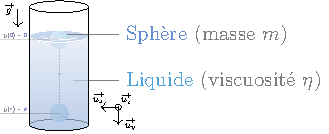
\includegraphics{Figures/sphere-in-liquid.pdf}
                \end{center}
            \end{minipage}
            
            Le mouvement est rectiligne, selon l'axe porté par $\vec{u_y}$. On pose $v_y = \vec{v} \cdot \vec{u_y}$ et on applique le \textit{principe fondamental de la dynamique} sur cet axe :
            %
            \[ m\dfrac{\dif v_y}{\dif t} = mg - 6\pi\eta r v_y \qquad\text{soit}\qquad \dfrac{\dif v_y}{\dif t} + \dfrac{6\pi\eta r}{m}v_y = g\]
            %
            Cette équation différentielle du premier ordre a pour solution :
            %
            \[ v_y\p{t} = A\exp{-\dfrac{6\pi\eta r}{m}t} + \dfrac{m}{6\pi\eta r}g \qquad\text{avec} \ A \ \text{une constante à déterminer}\]
            %
            La condition initiale $v_y\p{0} = 0$ livre $A = -\dfrac{mg}{6\pi\eta r}$ d'où $v_y\p{t} = \dfrac{mg}{6\pi\eta r}\p{1 - \exp{-\dfrac{6\pi\eta r}{m}t}}$. On intègre :
            %
            \[ y\p{t} = \dfrac{mg}{6\pi\eta r}\intc{t + \dfrac{m}{6\pi\eta r}\exp{-\dfrac{6\pi\eta r}{m}t}} + B \qquad\text{avec} \ B \ \text{une constante à déterminer}\]
            %
            Pour de grandes valeurs de $\tau$, on a alors $y\p{\tau} \approx \dfrac{mg}{6\pi\eta r}\tau$, donc pour $y\p{\tau} = h$ on obtient $h = \dfrac{mg\tau}{6\pi\eta r}$, d'où :
            %
        }
        %
        \nobefore\yesafter
        %
        \boxansconc{
            \[ \eta = \dfrac{mg\tau}{6\pi rh}\]
        }
        %
        \yesbefore
        
        \item On mesure $m = \SI{1.00}{\g}$ avec $u\p{m} = \SI{0.01}{\g}$, $m\tau= \SI{1.00}{\s}$ avec $u\p{\tau} = \SI{0.05}{\s}$, $r = \SI{1.0}{\mm}$ avec $u\p{r} = \SI{0.1}{\mm}$. On prendra $g = \SI{9.81}{\m \cdot \s^{-2}}$. Donner et encadrer la valeur de $\eta$.
    \end{enumerate}
    
    \subsection{}
    
    La mise en équation de la tension de sortie de l'oscillateur à pont de \textsc{Wien} donne le résultat suivant :
    %
    \[ \dfrac{\dif^2 V_\text s}{\dif t^2} + 2\Omega_0 \alpha + \Omega_0^2V_\text s = 0 \qquad\text{où} \ \Omega \ \text{et un réel positif et} \ \alpha \ \text{est un réel}\]
    %
    Discuter la stabilité du système et les différentes solutions possibles en fonction de $\alpha$.
    
    \boxans{
        Il s'agit d'un système [décrit pas une équation différentielle] du deuxième ordre. On considère donc 
    }
    
    \subsection{}
    
    Un liquide placé dans un récipient cylindrique de section $S$, occupe au repos un volume caractérisé par une hauteur $h_0$. On fait tourner le récipient autour de son axe à vitesse angulaire constante. Une fois le régime permanent établi, la surface libre du liquide prend une forme parabolique d'équation $z = ar^2 + h$.
    
    \begin{enumerate}
        \item Exprimer $h$ en fonction de $h_0$ et des autres données de l'énoncé.
        
        \boxansconc{
            On suppose que l'eau est une phase incompressible et indilatable (PCII). 
        }
        
        \item Une jarre sphérique de rayon $R$ contient une hauteur $h_0$ d'eau. Le volume qui s'évapore par unité de temps est proportionnel à la surface eau-air. Déterminer le temps pour que la jarre soit vide en fonction du coefficient de proportionnalité.
    \end{enumerate}

    \chapter{Électronique, analyse harmonique d'un signal périodique, numérisation}
    
    \subsection{}
    
    \begin{minipage}{0.48\linewidth}
         Soit le circuit suivant :\medskip
    
    A l'instant initial, le condensateur de capacité $C$ est chargé avec la charge $Q_0$, celui de capacité $C'$ est déchargé.
    \end{minipage}
    %
    \hfill
    \begin{minipage}{0.48\linewidth}
            \begin{center}
        \begin{circuitikz}
            \draw (0, 0) --++(0, 2) to[C, l=$C$, v=$u_C\p{t}$] ++(3, 0) to[C, l=$C'$, v=$u_{C'}\p{t}$] ++(3, 0) to[short, i=$i\p{t}$] ++(0, -2) to[R, l=$R$, v=$u_R\p{t}$] ++(-6, 0);
        \end{circuitikz}
    \end{center}
    \end{minipage}

    \begin{enumerate}
        \item Établir l'expression de $i\p{t}$, le courant qui parcourt le circuit au cours du temps.
        
        \boxans{
        
        }
        
        \item Quelle est l'énergie dissipée par le circuit ? Comparer avec les énergies initiales et finales ?
        
        \boxans{
        
        }
    \end{enumerate}
    
    \subsection{}
    
    \subsection{}
    
    La tension $u\p{t}$ a la forme ci-dessous :
    
    DESSIN 
    
    On a $T < RC$ et $\alpha < 1$. Déterminer les allures de $u_1$ et $u_2$.
    
    \boxans{
    
    }
    \subsection{}

    \subsection{}

    \subsection{}
    % je sais pas dessiner le circuit (xD)
    \begin{enumerate}
        \item \(e(t) = e_0\cos(\omega t)\) On veut que la composante sinusoïdale en \(A\) soit atténué de 40 dB. En déduire une condition sur R, C et \(\omega\), on supposera cette condition vérifiée par la suite.

        \boxans{
            Sur une sinusoïde : \[V_B = \frac{Z_C}{R + Z_C}V_A \text{donc} H = \frac{1}{1 + jRC\omega}\]
            Donc sur l'entrée souhaitée \(V_A = ke_0^2\cos^2(\omega t) = \dfrac{ke_0^2}{2} + \dfrac{ke_0^2\cos(2\omega t}{2}\) ainsi la sortie de la composante sinusoïdale est \[V_B = \dfrac{1}{\sqrt{1+ 4(Rc\omega)^2}}\dfrac{ke_0^2}{2}\cos(2 \omega t - \arctan(2RC\omega))\]
            On a enfin par définition \(G_{dB} = 20\log\left|\dfrac{V_B}{V_A}\right|\) donc 
            \(G_{dB} = -40 \Leftrightarrow \omega \geq 100 \omega_0\)
        }

        \item Déterminer \(s(t)\)

        \boxans{
            On a trivialement \(s^2(t) = k^{-1}V_B\) or \(\omega_0 << \omega\) donc 
            \(V_B \equiv V_B(0) = k\dfrac{e_0^2}{2}\) donc \(s(t) = \pm \dfrac{e_0}{2}\)
        }

        \item Le dipôle \(D\) est une diode telle que \(s(t) = \lnot i(t)\)

        \boxans{
            La diode force la tension positive, donc \(s(t) = \dfrac{\left|e_0\right|}{\sqrt{2}}\)
        }

        \item Montrer que ce montage fonctionne comme un voltmètre. Est-ce une mesure AC ou DC ? Le fonctionnement serait-il modifié si le signal d'entrée n'était pas sinusoïdal ?

        \boxans{
            On observe que \(s(t)\) est bel et bien la valeur RMS de \(e(t)\) donc ce montage se comporte bien comme un voltmètre, on est en DC car la valeur moyenne a de l'influence sur le résultat final.
        }
    \end{enumerate} 


    \subsection{}
    % je sais pas dessiner le circuit
    \begin{enumerate}
        \item Déterminer et caractériser la fonction de transfert \(H(j\omega\) du circuit.

        \boxans{
            En utilisant le théorème de \textsc{Millman} on trouve \(H = \dfrac{1 - jRC\omega}{1 + jRC\omega}\) ainsi \(G(\omega) = 1\) et \(\varphi = 2 tan^{-1}(RC\omega)\) le filtre est donc déphaseur.
        }


        \item La tension d'entrée \(v_e(t)\) est la fonction créneau définie par \(f(t) = \dfrac{4E}{\pi} \sum_{i=1}^{+\infty} \dfrac{1}{2i+1} \sin \left( 2 \pi (2i+1) \dfrac{t}{T} \right)\) avec \(T >> \tau = RC\) quelle est la tension de sortie ?

        \boxans{
            On a par définition la sortie \(s(t) = e_0\left|H_0\right| + \sum_{n=1}^{\infty} e_n \left|H(jn\omega)\right|\cos\left(n\omega t + \varphi_n + \arg(H(jn\omega))\right)\) \\
            Dans notre cas on a donc \[s(t) = \dfrac{4E}{\pi}\sum_{n=1}^{\infty} \dfrac{1}{2n+1} \sin\left((2n+1)\omega(t - 2\tau)\right)\]

            La tension de sortie est donc simplement celle d'entrée déphasée d'environ -180° comme \(T>>\tau\) on est à l'asymptote.
        }
    \end{enumerate}
    
    \chapter{Changement de référentiel et dynamique en référentiel non galiléen}
    
    \subsection{}
    
    Dans le cas d'un référentiel $\bcR_2$ en mouvement quelconque par rapport au référentiel $\bcR_1$, utiliser la dérivée covariante pour établir les lois de composition des vitesses et des accélérations dans le cas général. Retrouver l'expression de ces lois dans le cas d'un mouvement de translation puis de rotation uniforme.
    
    \subsection{Bifurcation}
    
    Un cercle de rayon $R$ tourne autour de son diamètre vertical à la vitesse angulaire constante $\omega$. Une petite bague peut coulisser sans frottements le long de ce cercle. Quelles sont les positions d'équilibre ? Stabilité ? Expliquer le titre.
    
    \boxans{
        $R_1\p{C, \vec{e_x}, \vec{e_y}, \vec{e_z}}$ et $\bcR_2\p{C, \vec{u_\rho}, \vec{u_\alpha}, \vec{u_\gamma}}$.
        
        $\vec{R}$ sans composante tangentielle car pas de frottement.
        
        
        
        Si $\dfrac{G}{R\omega^2} < 1$, alors les positions d'équilibre sont $\pm \arccos{}$
    }
    
    \chapter{Frottement solide}
    
    \subsection{}
    
    Une caisse cubique est posée sur un sol incliné d'un angle $\alpha$ par rapport à l'horizontale. On appelle $f = \tan \varphi$ le coefficient de frottement caisse-sol. On augmente progressivement $\alpha$, à quelles conditions l'équilibre est-il rompu ? La caisse glisse-t-elle ou bascule-t-elle ?
    
    
    
    \subsection{}
    
    \begin{minipage}{0.48\linewidth}
        Soit le système mécanique ci-contre.\newline
        
        Le fil et la poulie sont de masses négligeables. La masse $M$ glisse sur le plan horizontal avec un coefficient de frottement $f$.\medskip
        
        On lâche le système sans vitesse initiale alors que la masse $m$ est à une altitude $h$ du plan inférieur.  
    \end{minipage}
    %
    \hfill
    %
    \begin{minipage}{0.5\linewidth}
        \centering
        \begin{tikzpicture}
            \draw[very thick] (0.5, 0) --++(4, 0) --++(0, -4) --++(3, 0); %sol
            
            \draw (1, 0) -- (1, 1) -- (2.5, 1) -- (2.5, 0); %boite M
            \node at (1.75, 1.25) {$M$}; %label M
            
            \draw[very thick] (4.5, 0) --++(0.2, 0.2); % Petit truc avant la poulie
            
            \draw (2.5, 0.47) -- (4.8, 0.47); %Fil M -> Poulie
            \draw (4.97, 0.3) --++(0, -1.3); %Fil Poulie -> m
            
            \node[circle,draw,minimum size=0.3,very thick] at (4.8,0.3){}; %Poulie
            
            \draw (4.7, -1) --++(0.6, 0) --++(0, -0.6) --++(-0.6, 0) --++(0, 0.6);
            
            \node at (5.6, -1.3) {$m$};
        \end{tikzpicture}
    \end{minipage}
    
    \begin{enumerate}
        \item Montrer que le mouvement de $M$ peut être décomposé en deux phases. Déterminer l'évolution de sa vitesse et établir l'expression de $v_\text{max}$ en fonction des paramètres du problème.
        
        \item Déterminer le coefficient de frottement $f$ en fonction de la distance $\ell$ parcourue par $M$.
        
        \item Reprendre l'étude en supposant que la poulie possède un rayon $r$ et un moment d'inertie $J$ non négligeables.
        
        \item On néglige $J$ et $r$. On recommence l'expérience en plaçant sous la masse $m$ un ressort de raideur $k$ et de longueur à vide $\ell_0$. Il est placé verticalement avec l'une de ses extrémités fixées sur le plan inférieur. Étudier les différentes phases du mouvement.
    \end{enumerate}
    
    \subsection{}
    
    \begin{minipage}{0.48\linewidth}
        Un ca
    \end{minipage}
    %
    \hfill
    %
    \begin{minipage}{0.5\linewidth}
        \centering
        \begin{tikzpicture}
            %\draw[very thick] (0, 0) --++ (4, 0) --++(0, 1) --++(-1, 1) --++(0, -2);
            
            \draw [fill=main3!30!black!10] (0,0) --++ (4, 0) --++ (0, 0.75) --++(-0.25, 0.75) --++(-0.75, 0) --++(0, -1.2) --++(-2.7, 0) --(0, 0); 
            \node[circle,draw,minimum size=0.5cm,thin,fill=main3!30] at (0.75,-0.1){};
            \node[circle,draw,minimum size=0.5cm,thin,fill=main3!30] at (3.25,-0.1){};
            
            \fill[fill,pattern=north east lines] (-0.2, -0.35) --++(4.5, 0) --++(0, -0.2) --++(-4.5, 0);
            \draw[] (-0.2, -0.35) --++(4.5, 0);
        \end{tikzpicture}
    \end{minipage}
    
    
\end{document}
% lim francois = paien ~ paysan ===> golem